% !TeX program = xelatex
% !TEX encoding = UTF-8 Unicode

\documentclass[9pt]{article}
\usepackage{hyperref}
\usepackage{ulem} 
\usepackage{mathtools}
\usepackage{enumitem}
\usepackage{color,soul}
\usepackage{inputenc}
\usepackage[margin=2.75cm]{geometry}
\usepackage{xcolor}
\usepackage{listings}

% TODO Modificare questi parametri per scrivere un bash più bello

\lstset{basicstyle=\ttfamily,
	showstringspaces=false,
	commentstyle=\color{blue},
	keywordstyle=\color{red}
}
% \lstset{
% 	language=bash,
% 	basicstyle=\ttfamily
% }

\begin{document}

\title{Shell Scripting 2020: Week 3}
\author{\textbf{Stefan Ciprian Voinea}\\Student number: 015383372}
\maketitle

%\begin{figure}[h!]
%	\centering
%	\includegraphics[width=12cm]{autoconfiguration.png}
%	\caption{IPv6 Autoconfiguration example}
%	\label{fig:autoconfig}
%\end{figure}

\begin{enumerate}
	
	\setcounter{enumi}{16}
	
	\item \textbf{Introduction to variables}
	
        \begin{lstlisting}[breaklines=true]
HISTCMD=The history number, or index in the history list, of the    current command.  If HISTCMD is unset, it loses its special properties, even if it is subsequently reset.
HOME=The home directory of the current user; the default argument for the cd builtin command.  The value of this variable is also used when performing tilde expansion.
PWD=The current working directory as set by the cd command.
		\end{lstlisting}
    
    \item \textbf{Special Shell variables}
    
        Contents of the \texttt{task18\_echo.sh} file:
        \begin{lstlisting}
echo $@
        \end{lstlisting}

        Output of the execution:

        \begin{figure}[h!]
            \centering
            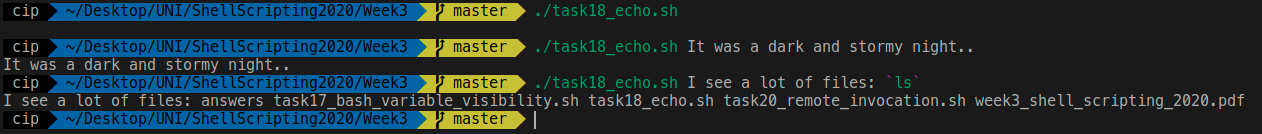
\includegraphics[width=\linewidth]{img/18.png}
        \end{figure}

    \item \textbf{The difference between Bash and Bash}
    
        Contents of the \texttt{task19\_bash\_variables.sh} file:
        \begin{lstlisting}
myvar="can you see me?"

echo "Variable in shell 1: $myvar"
echo "Shell 1 PID: $$"

echo ""

bash -c 'echo "Variable in shell 2: $myvar" ; echo "Shell 2 PID: $$"'
        \end{lstlisting}

        Output of the execution:

        \begin{figure}[h!]
            \centering
            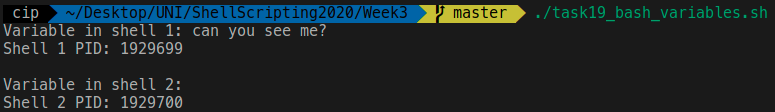
\includegraphics[width=\linewidth]{img/19.png}
        \end{figure}

    \item \textbf{Remote invocation}

        Contents of the \texttt{task20\_remote\_invocation.sh} file:
        \begin{lstlisting}
ssh stefvoin@$1 $2
        \end{lstlisting}

        Output of the execution:

        \begin{figure}[h!]
            \centering
            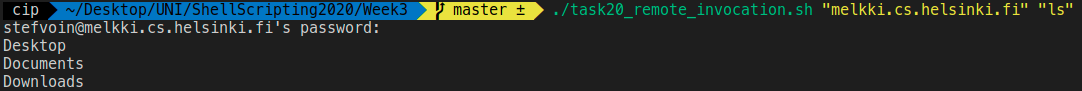
\includegraphics[width=\linewidth]{img/20.png}
        \end{figure}

    \item \textbf{Tar}
        
        The commands I used for creating the tars:
        \begin{lstlisting}
tar cf scriptz.tar.bz2 $(find ../ -type f -name "*.sh" -o -name "*.jpg")
tar cf scriptz.tar.gz $(find ../ -type f -name "*.sh" -o -name "*.jpg")
        \end{lstlisting}

        File sizes in bytes:
        \begin{figure}[h!]
            \centering
            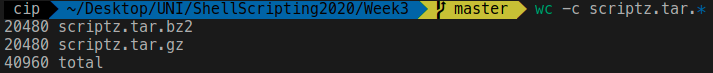
\includegraphics[width=\linewidth]{img/21_1.png}
        \end{figure}

        For creating the archives with \texttt{bzip2} ... 
        \begin{lstlisting}[breaklines=true]
bzip2 -c $(find ../ -type f -name "*.sh") > scriptz_arkive.bz2 | bzip2 -c $(find ../ -type f -name "*.jpg") >> scriptz_arkive.bz2
        \end{lstlisting}

        ... and gzip:
        \begin{lstlisting}[breaklines=true]
gzip -r -c $(find ../ -type f -name "*.sh") > scriptz_arkive.gz | gzip -c $(find ../ -type f -name "*.jpg") >> scriptz_arkive.gz
        \end{lstlisting}

    \item \textbf{Local and network file systems}
    
        Name of the system: \texttt{cip-tp} (\texttt{echo \$HOST})\\
        Operating system: \texttt{Ubuntu 20.04.1 LTS} (\texttt{lsb\_release -a})\\
        File system of the host: \texttt{ext4} (\texttt{df -Th})
        
    \item \textbf{Fetch and extract}
        
        The command I use to solve this exercise was:
        \begin{lstlisting}[breaklines=true]
wget -O - https://wiki.helsinki.fi/download/attachments/124126879/lost24-monitor-temps-and-fans-v2.tar.bz2 | tar -xvjf -
        \end{lstlisting}

    \item \textbf{Doing your business somewhere else}
    
        The command I use to solve this exercise was:
        \begin{lstlisting}[breaklines=true]
ssh stefvoin@melkki.cs.helsinki.fi "wget -O - https://wiki.helsinki.fi/download/attachments/124126879/lost24-monitor-temps-and-fans-v2.tar.bz2" | tar -xvjf -
        \end{lstlisting}
    
    \item \textbf{GREP and CUT}

        Contents of the \texttt{task25\_unique\_temperatures.sh} file:
        \begin{lstlisting}[breaklines=true]
record_date="2011.12.25"
workdir="/home/cip/Desktop/UNI/ShellScripting2020/Week3/lost24/monitor/$record_date"

rm -f temps.txt
rm -f temps_tmp.txt

for dir in `find $workdir -type d`
do
    # ls $dir/hp-temps.txt
    grep "PROCESSOR_ZONE *[0-9][0-9]C" $dir/hp-temps.txt -s | cut -b 32-34 >> temps_tmp.txt
done

sort temps_tmp.txt | uniq >> temps.txt

rm temps_tmp.txt

cat temps.txt
        \end{lstlisting}

        Output of the execution:
        \begin{lstlisting}
22C
23C
24C
25C
26C
27C
28C
29C
30C
31C
        \end{lstlisting}

    \item \textbf{Don't run with the scissors}

        Contents of the \texttt{task26\_csv\_temp.sh} file:
        \begin{lstlisting}
./task25_unique_temperatures.sh

echo ""

sed 's/ +/ /g; s/\s+/,/g; s/\//,/g' temps.txt > temps.csv

cat temps.csv
        \end{lstlisting}

    \item \textbf{Too long to read}
    
        Output of the wrong command:
        \begin{figure}[h!]
            \centering
            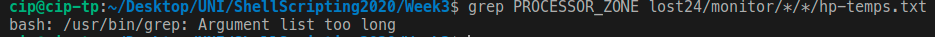
\includegraphics[width=\linewidth-2cm]{img/27_1.png}
        \end{figure}        

        The command for finding all the files from 2011.11 is:
        \begin{lstlisting}
find lost24/monitor -wholename "*/*/hp-temps.txt"
        \end{lstlisting}

        Output of the command:
        \begin{figure}[h!]
            \centering
            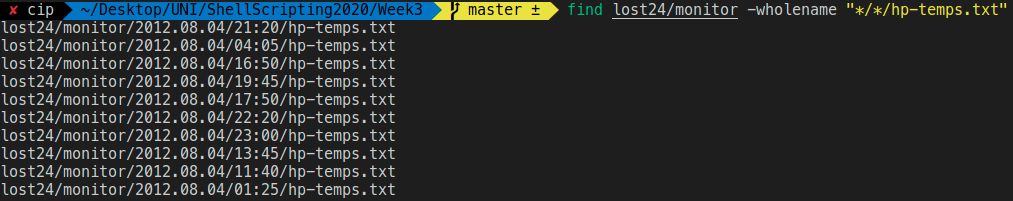
\includegraphics[width=\linewidth-2cm]{img/27_2.png}
        \end{figure}     
    
    \item \textbf{Escape as a true friend}
    
        Output of the commands:
        \begin{figure}[h!]
            \centering
            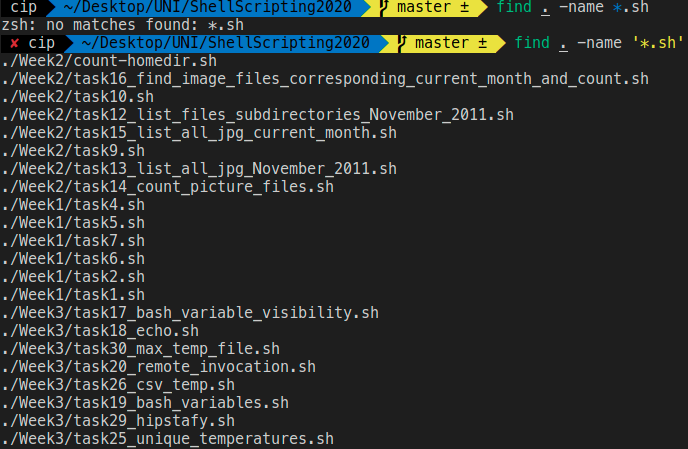
\includegraphics[width=\linewidth-2cm]{img/28.png}
        \end{figure}

    \item \textbf{The Immelmann}
    
        Contents of the \texttt{task29\_hipstafy.sh} file:
        \begin{lstlisting}[breaklines=true]
input_dir="$1"

output_dir=$input_dir/OUTPUT
mkdir -p $output_dir

images=`find $input_dir -type f -name "*.jpg"`

for image in $images
do
    image_name=`basename $image`
    image_prefix=${image_name%.jpg}
    output_file=$output_dir/$image_prefix-hipstah.jpg
    echo "Converting ... $output_file" 
    convert -sepia-tone 60% +polaroid $image $output_file 
done

echo "DONE!"
        \end{lstlisting}    

        Output of the execution:
        \begin{figure}[h!]
            \centering
            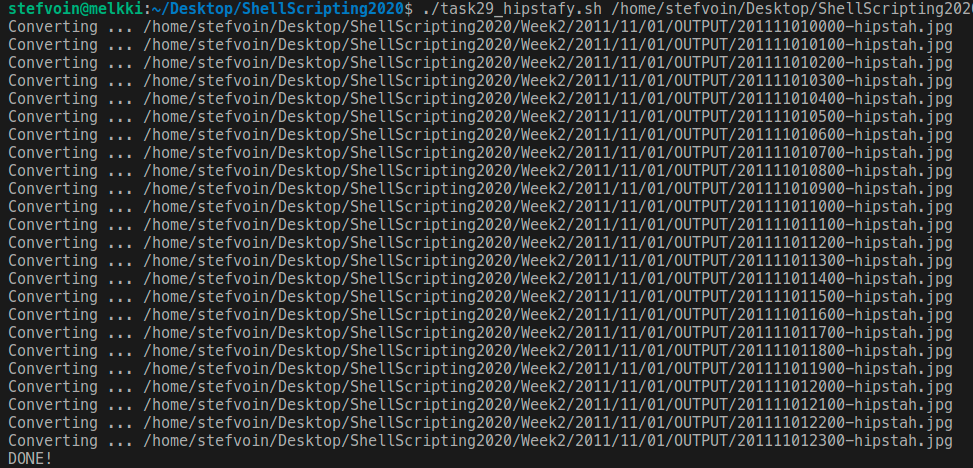
\includegraphics[width=15cm]{img/29_1.png}
        \end{figure}
        \vspace{-.5cm}
        \begin{figure}[h!]
            \centering
            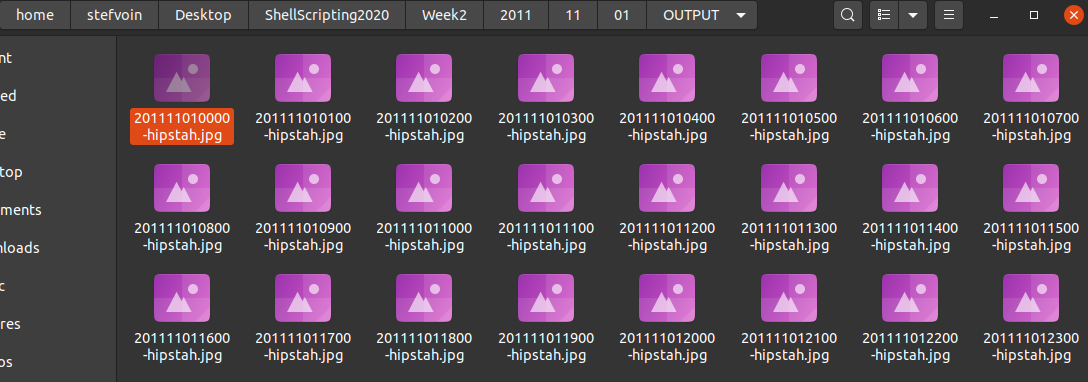
\includegraphics[width=15cm]{img/29_2.png}
        \end{figure}
        \vspace{-.5cm}
        \begin{figure}[h!]
            \centering
            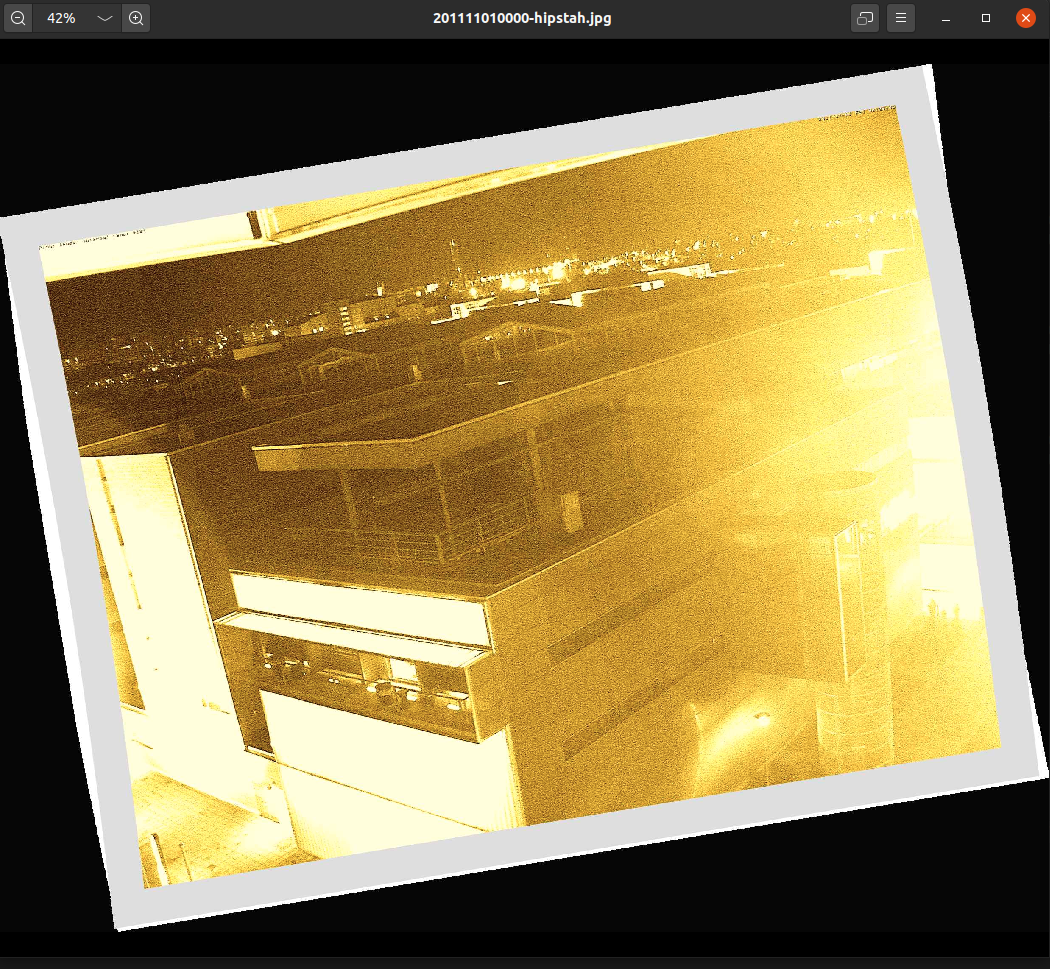
\includegraphics[width=6.5cm]{img/29_3.png}
        \end{figure}

    \newpage
    \item \textbf{Testing}
    
        Contents of the \texttt{task29\_hipstafy.sh} file:
        \begin{lstlisting}
dirs=`find lost24/monitor/ -type d -name "2011.11.*"`
files=`find $dirs -type f -name "*temps.txt"`

max_temp_file=""
max_temp=0

for file in $files
do
    temp=`grep "PROCESSOR_ZONE *[0-9][0-9]C" $file -s | cut -b 32-33`
    
    echo "File: $file"
    echo "Temperature: $temp"

    if [ $temp -gt $max_temp ]
    then
        max_temp=$temp
        max_temp_file=$file
    fi

done

echo "Max temp: $max_temp"
echo "Max temp file: $max_temp_file"
        \end{lstlisting}

        Partial output of the execution:
        \begin{figure}[h!]
            \centering
            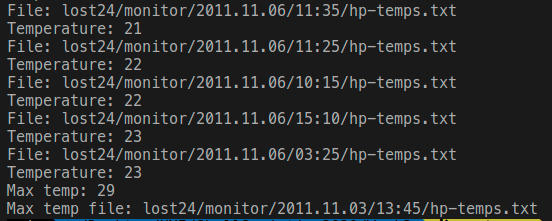
\includegraphics[width=12cm]{img/30.png}
        \end{figure}

\end{enumerate}

\end{document}